\documentclass[twocolumn,a4j]{jsarticle}
\bibliographystyle{junsrt}

\setlength{\topmargin}{-20.4cm}
\setlength{\oddsidemargin}{-10.4mm}
\setlength{\evensidemargin}{-10.4mm}
\setlength{\textwidth}{18cm}
\setlength{\textheight}{26cm}

\usepackage[top=15truemm,bottom=20truemm,left=20truemm,right=20truemm]{geometry}
\usepackage[latin1]{inputenc}
\usepackage{amsmath}
\usepackage{amsfonts}
\usepackage{amssymb}
\usepackage[dvipdfmx]{graphicx}
\usepackage[hang,small,bf]{caption}
\usepackage[subrefformat=parens]{subcaption}
\usepackage[dvipdfmx]{color}
\usepackage{listings}
\usepackage{listings,jvlisting}
\usepackage{geometry}
\usepackage{framed}
\usepackage{color}
\usepackage[dvipdfmx]{hyperref}
\usepackage{ascmac}
\usepackage{enumerate}
\usepackage{tabularx}
\usepackage{cancel}
\usepackage{scalefnt}
\usepackage{overcite}
\usepackage{otf}
\usepackage{multicol}
\usepackage[geometry]{ifsym}

\renewcommand{\figurename}{Fig.}
\renewcommand{\tablename}{Table }

\hypersetup{%
    hidelinks %リンクの色消し
}

\lstset{
basicstyle={\ttfamily},
identifierstyle={\small},
commentstyle={\smallitshape},
keywordstyle={\small\bfseries},
ndkeywordstyle={\small},
stringstyle={\small\ttfamily},
frame={tb},
breaklines=true,
columns=[l]{fullflexible},
xrightmargin=0zw,
xleftmargin=3zw,
numberstyle={\scriptsize},
stepnumber=1,
numbersep=1zw,
lineskip=-0.5ex
}

% キャプション後ろのダブルコロンを消す
\makeatletter
\long\def\@makecaption#1#2{%
  \vskip\abovecaptionskip
  \iftdir\sbox\@tempboxa{#1\hskip1zw#2}%
    \else\sbox\@tempboxa{#1 #2}%
  \fi
  \ifdim \wd\@tempboxa >\hsize
    \iftdir #1\hskip1zw#2\relax\par
      \else #1 #2\relax\par\fi
  \else
    \global \@minipagefalse
    \hbox to\hsize{\hfil\box\@tempboxa\hfil}%
  \fi
  \vskip\belowcaptionskip}
\makeatother


\makeatletter
\def\@maketitle
{
\begin{center}
{\LARGE \@title \par}
\end{center}
\begin{flushright}
{\large \@date}\\
{\large M2 \@author}
\end{flushright}
\par\vskip 1.5em
}
\makeatother

\author{来代 勝胤 / KITADAI Masatsugu}
\title{令和5年度 6月度 月例報告書}
\date{2023/06/28}

\begin{document}
\columnseprule=0.1mm
\maketitle

\section*{報告内容}
\begin{enumerate}[1.]
  \item 対応枚数差の組み合わせの変更
  \item 数値シミュレーション結果
  \item 7月の予定
\end{enumerate}

\section*{進捗報告}
今月は,ISTPの原稿作成に向けた
数値シミュレーション結果の整理および
計測アルゴリズムの検討を行った.

\section{対応枚数差の組み合わせの変更}
\subsection{対応枚数による相間係数の推移}
枚数差の組み合わせによる各値の推移を調べた.
撮影画像に対して Fig.1 のように $y,z$ 方向に 10 [mm] 間隔で格子点を配置し,
その点上での $y$方向速度 $v$ [mm/s], $z$方向速度 $w$ [mm/s],および
PTVプログラムで算出される相互相間係数 $R$ [-] の変化をFig.2に示す.
また,Fig.1で取り上げた代表点について,青(40,10)は渦成分を大きく含むと考えられる位置,
赤(50,20)は渦の中心付近の位置,紫(90,20)は渦の影響が少ないと考えられる位置
を選択している.Fig.2(a) は$R$のピークが$n=10$にあることに対して,
Fig.2(b) は$n=9$にあることがわかる,これより,主流方向の速度を考慮した
PTVアルゴリズムの作成が必要であることがわかる.\\

\begin{figure}[htbp]
  \footnotesize
  \begin{center}
    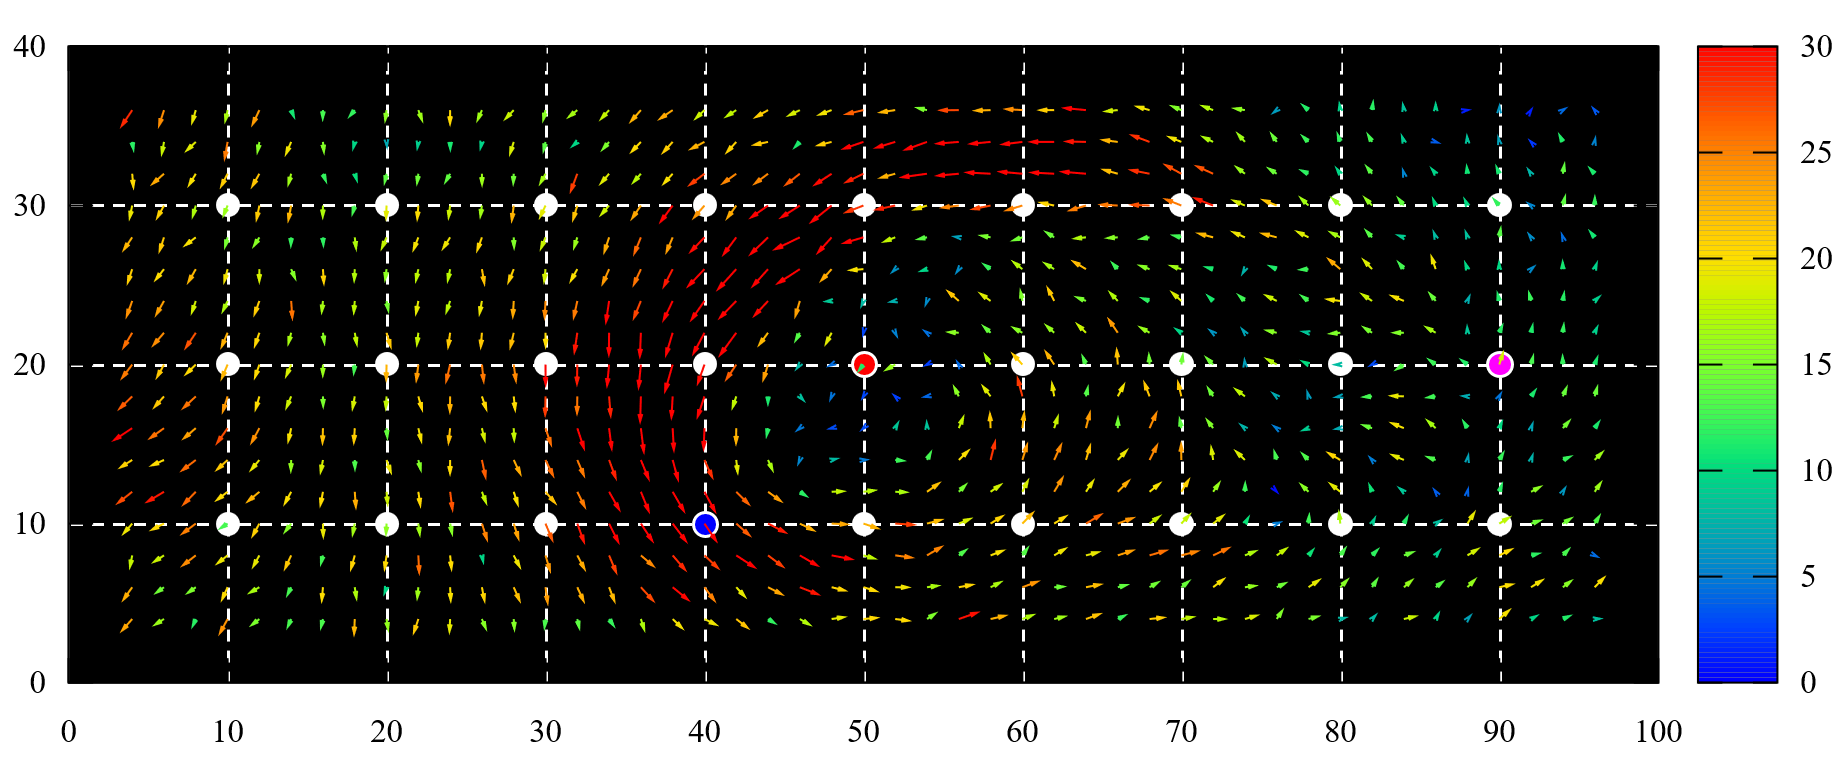
\includegraphics[width=80mm]{../images/vector_grid.png}
    \caption{Velocity vectors of delta wake : $n = 10$}
  \end{center}
\end{figure}

\subsection{格子点ごとの組み合わせの選択}
枚数差の組み合わせによる差異の検討を行った.
Fig.3 に,最大の相間係数をとる組み合わせを選択して
速度場を表現した結果を示す.
結果より,渦中心の対応枚数差$n$が大きくなっていることから
主流方向速度が低下していることがわかる.
また,渦中心から離れるごとに$n$の値が小さくなっており,
円状に分布していることからも妥当性の高い結果だと考えられる.
したがって,場所によって対応枚数差を変更する必要があることがわかった.

\begin{figure}[htbp]
  \footnotesize
  \begin{center}
    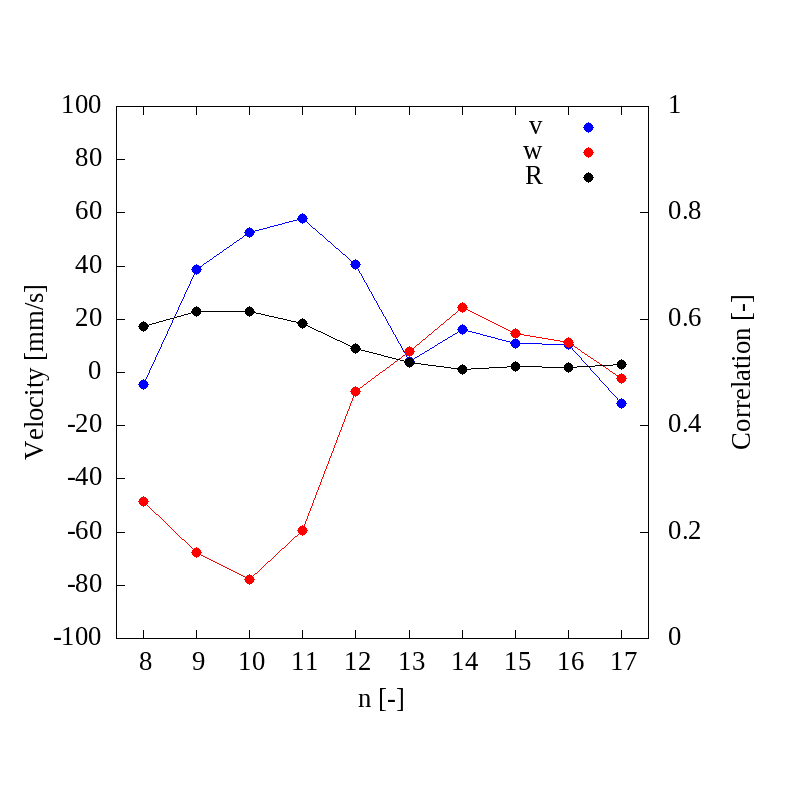
\includegraphics[width=62mm]{../images/x=40,y=10.png}
    \subcaption{Blue : $(y,z) = (40,10)$}
    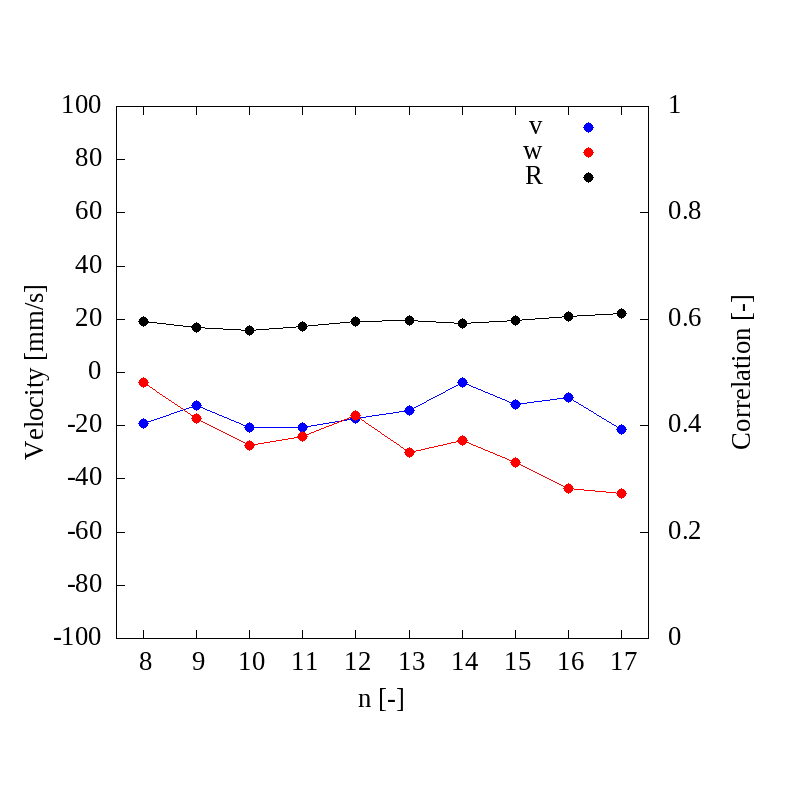
\includegraphics[width=62mm]{../images/x=50,y=20.png}
    \subcaption{Pink : $(y,z) = (90,20)$}
  \end{center}
  \caption{Value transition of $v$, $w$ and $R$}
  \vskip \baselineskip
  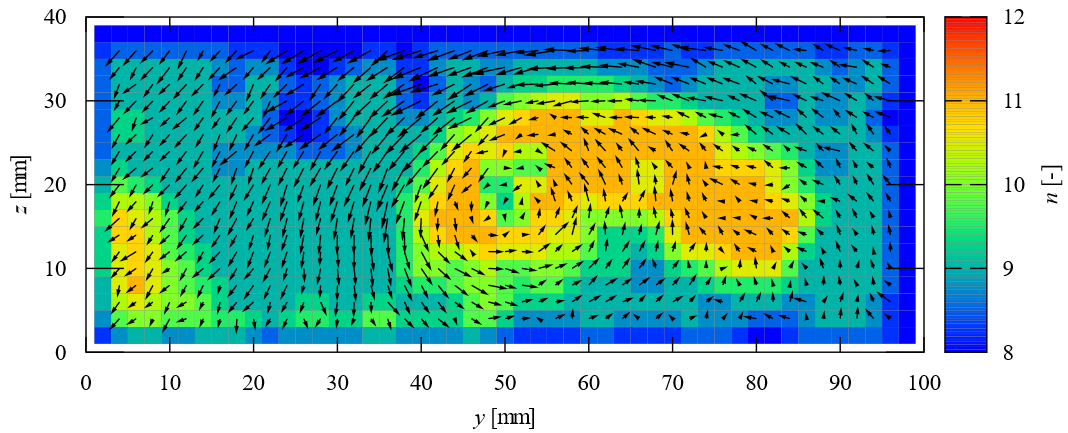
\includegraphics[width=80mm]{../images/velocity_and_vorticity.png}
  \caption{Velocity vectors of delta wake and selected $n$ }
\end{figure}

\newpage

\section{数値シミュレーションの結果}

\section{7月の予定}
\begin{itemize}
  \item ISTP 原稿提出 (6/30)
  \item タイヤモデル周りの流れ場測定実験
\end{itemize}

\end{document}